\documentclass{standalone}
\usepackage{tikz}
\usepackage{ctex,siunitx}
\setCJKmainfont{Noto Serif CJK SC}
\usepackage{tkz-euclide}
\usepackage{amsmath}
\usepackage{wasysym}
\usetikzlibrary{patterns, calc}
\usetikzlibrary {decorations.pathmorphing, decorations.pathreplacing, decorations.shapes,}
\begin{document}
\small
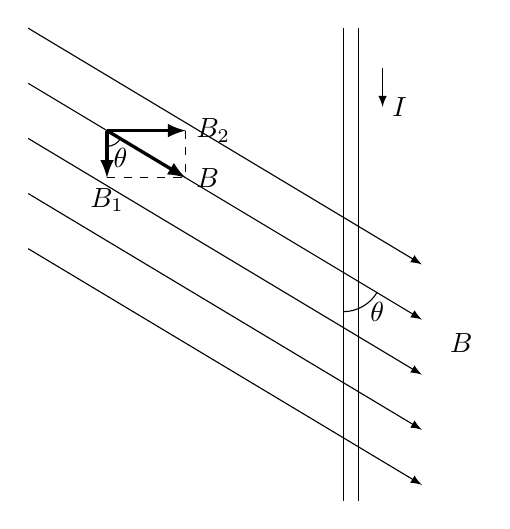
\begin{tikzpicture}[>=latex,scale=1]
  \draw (0,6)--(0,0);
  \draw (.2,6)--(.2,0);
  \draw[->] (.5,5.5)--(.5,5)node[right]{$I$};
  \foreach \x in {0,1,...,4}
  {
      \draw[->](-4,6-\x*.7)--(1,3-\x*.7);
  }
  \node at (1.5, 2){$B$};
  \draw (0,2.9-.5) arc (-90:-30:.5)node[below]{$\theta$};
  \draw[->, very thick] (-3,5.3-.6)--(-2,5.3-.6)node[right]{$B_2$};
  \draw[->, very thick] (-3,5.3-.6)--(-3,5.3-.6-.6)node[below]{$B_1$};
  \draw[->, very thick] (-3,5.3-.6)--(-2,5.3-.6-.6)node[right]{$B$};
  \draw[dashed] (-3,5.3-.6-.6)--(-2,5.3-.6-.6);
  \draw[dashed] (-2,5.3-.6)--(-2,5.3-.6-.6);
  \draw (-3,5.3-.6-.2) arc (-90:-30:.2)node[below]{$\theta$};
\end{tikzpicture}
\end{document}